\usetikzlibrary{arrows, positioning, fit}

\section{Reinforcement Learning Developments}

Recently, Sutton and Barto received the Turing Award for their contributions in developing the foundations of Reinforcement Learning. In regards of those contributions, they also adopt the concepts coming from other fields, such as Psychology and Neuroscience, as the study of true intelligence are coming from those fields. 

In RL, an agent have two main properties, i.e. to \textbf{percieve} and \textbf{act}. Likely, the future developments of AI will continue upon RL, after the development of the other subfields like in Supervised and Unsupervised Learning supporting the perceiving part of RL agent. Below is the illustration of RL scheme, where besides perceiving, an agent is also taking action, then the environment will evaluate those actions with evaluative feedback (with reward) rather than instructive feedback (giving the true answer) like in Supervised Learning.
\begin{figure}[h]
    \centering
    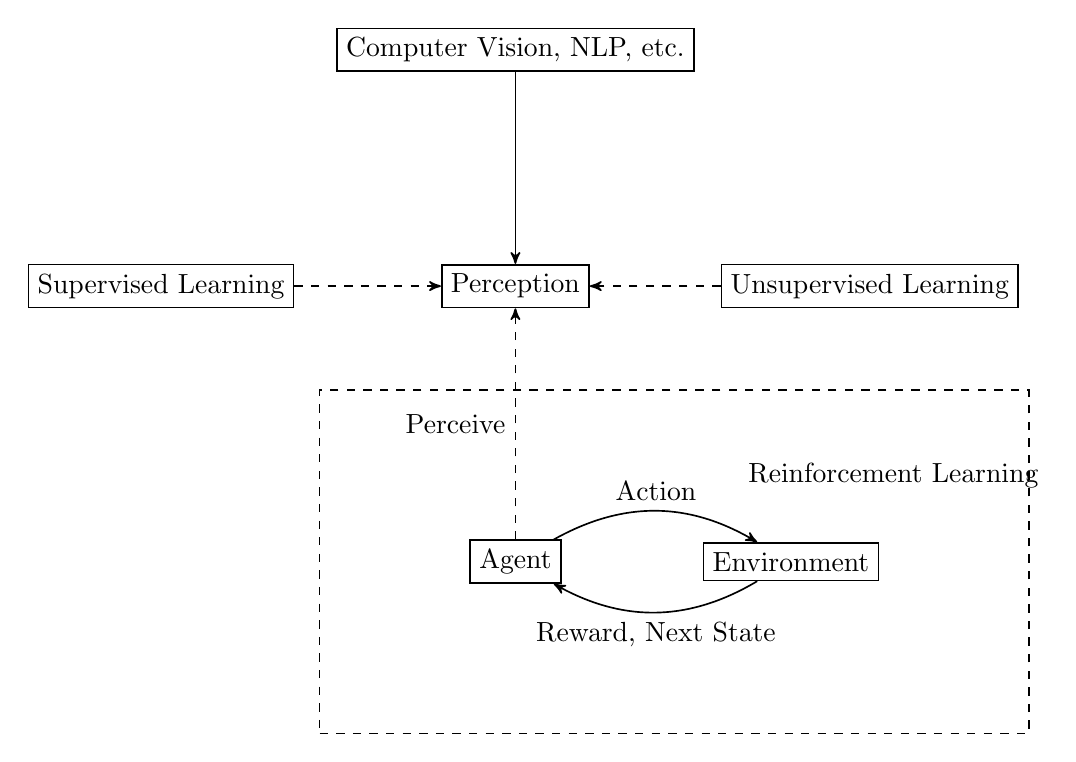
\begin{tikzpicture}[->, >=stealth', auto, semithick, node distance=3.5cm]
        \tikzstyle{state}=[fill=white,draw=black,text=black]

        \node[state]    (A)                     {Agent};
        \node[state]    (B) [right of=A] {Environment};
        \node[state]    (C) [above of=A, node distance=3.5cm] {Perception};
        \node[state]    (D) [above of=C, node distance=3cm] {Computer Vision, NLP, etc.};
        \node[state]    (E) [left of=C, node distance=4.5cm] {Supervised Learning};
        \node[state]    (F) [right of=C, node distance=4.5cm] {Unsupervised Learning};

        \node[draw, dashed, fit=(A) (B), inner sep=1.9cm, label={[label distance=-1.95cm]above right:{Reinforcement Learning}}] (RL) {};

        \path (A) edge [bend left] node[above] {Action} (B)
                  (B) edge [bend left] node[below] {Reward, Next State} (A)
                  (A) edge [->, dashed] node[left] {Perceive} (C)
                  (D) edge [->] node[right] {} (C) % Solid arrow for examples
                  (E) edge [->, dashed] node[below] {} (C) % Dashed arrow for ML schemes
                  (F) edge [->, dashed] node[below] {} (C); % Dashed arrow for ML schemes
    \end{tikzpicture}
    \caption{Reinforcement Learning Scheme with Perception}
    \label{fig:rl_scheme}
\end{figure}